\chapter{Graphs and tables}\label{ch:graphs-and-tables}


\section{Figures}\label{sec:figures}

\begin{figure}[ht]
\centering
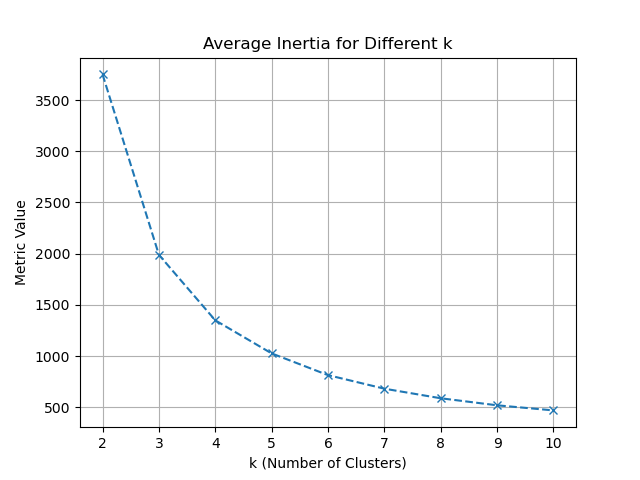
\includegraphics[width=0.8\textwidth]{Pictures/Average Inertia}
\caption{Graph for Average Inertia for K}
\label{fig:1}
\end{figure}

\begin{figure}[ht]
\centering
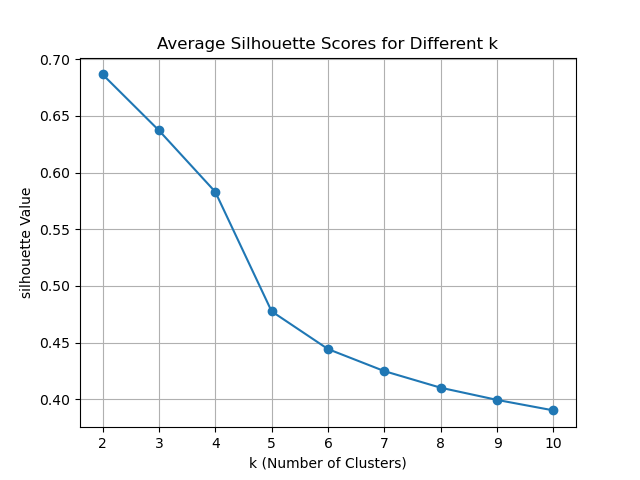
\includegraphics[width=0.8\textwidth]{Pictures/Average Silhouette Score}
\caption{Graph for Average Silhouette scores for K}
\label{fig:2}
\end{figure}

\begin{figure}[ht]
\centering
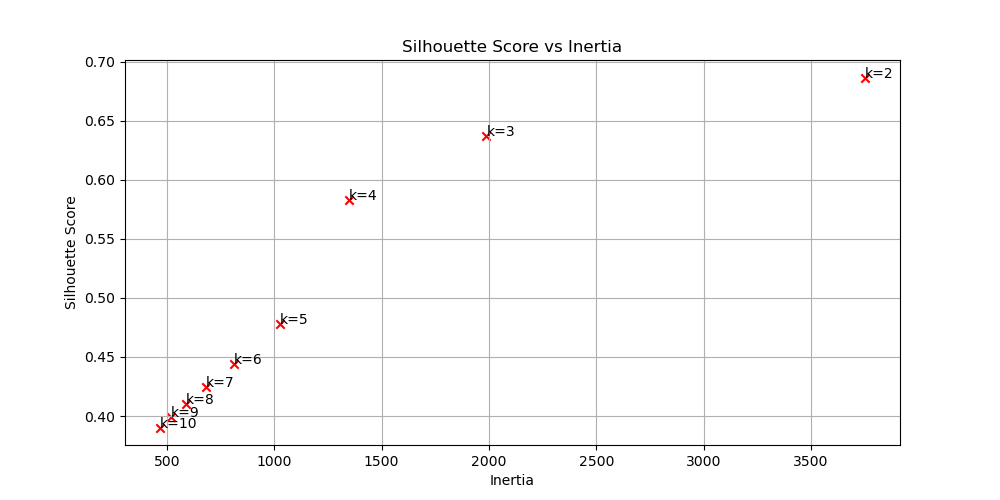
\includegraphics[width=0.5\textwidth]{Pictures/Silhouette score vs Inertia}
\caption{Graph for the Silhouette Score vs. Inertia}
\label{fig:3}
\end{figure}

\begin{figure}[ht]
\centering
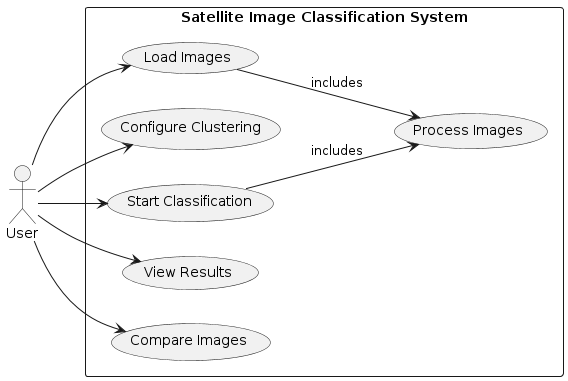
\includegraphics[width=0.4\textwidth]{Pictures/Use case Diagram}
\caption{Use case Diagram}
\label{fig:5}
\end{figure}

\begin{figure}[ht]
\centering
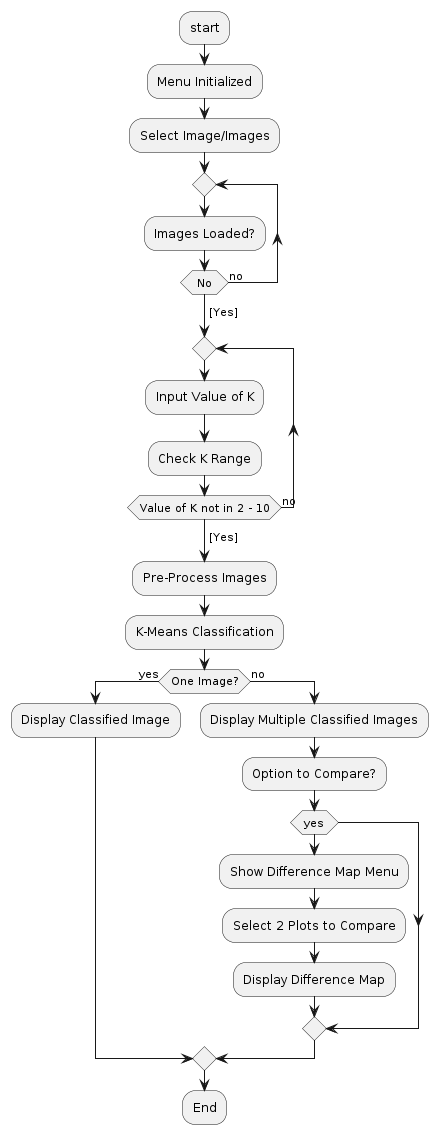
\includegraphics[width=0.4\textwidth]{Pictures/Program Flowchart}
\caption{}
\label{fig:6}
\end{figure}


\section{tables}\label{sec:tables}

\begin{table}[ht]
\centering
\caption{Feature List}
\begin{tabular}{|c|p{3cm}|p{4cm}|p{4cm}|}
\hline
\textbf{Feature Number} & \textbf{Feature Name} & \textbf{Feature Description} & \textbf{Acceptance Test} \\ \hline
1 & Load Satellite Imagery & Users should be able to upload and store satellite images & Users can upload images in supported formats (e.g., JPG). The system confirms successful uploads  \\ \hline
2 & View Images & Users should be able to view and manage their uploaded satellite images & All uploaded images are displayed in the user dashboard with options to zoom and pan\\ \hline
3 & Configure classification & Users should be able to configure parameters for classification & Users can select and set parameters such as number of clusters\\ \hline
4 & Start Classification & Users should be able to initiate the classification process on selected images & Classification process starts, and the system displays processing status.\\ \hline
5 & View Classification Results & Users should be able to view and analyze the results of image classifications & Results, including cluster maps and metrics are displayed for user analysis. \\ \hline
6 & Change Detection & Users should be able to compare classification results over time & comparison interface allows user to view a diff map of the two areas with the differences highLighted\\ \hline
\end{tabular}\label{tab:1}
\end{table}


\begin{table}[ht]
\centering
\caption{Test Descriptions}
\begin{tabular}{|c|p{3cm}|p{5cm}|c|}
\hline
\textbf{Test Number} & \textbf{Test Name} & \textbf{Test Description} & \textbf{Pass or Fail} \\ \hline
1 & File Format Compatibility Test & Upload a file which is jpg or png & Pass \\ \hline
2 & File Size and Resolution Test & Upload a very large Image & Pass \\ \hline
3 & Corrupted File Handling & Upload a corrupted image file & Fail \\ \hline
4 & Multi-file Upload Test & Upload multiple Files at once & Pass \\ \hline
6 & Upload Limits and Restrictions & Upload as many files as You can, should be able to & Pass \\ \hline
\hline
\end{tabular}\label{tab:2}
\end{table}